\chapter{The HADES detector}
\label{chapter:detector}
The \textbf{H}igh \textbf{A}cceptance \textbf{D}i-\textbf{E}lectron \textbf{S}pectrometer (HADES) \cite{Agakishiev:2009am} is located in the GSI Helmholtzzentrum f{\"u}r Schwerionenforschung. The HADES detector was designed for various measurements with an especial emphasis on di-electron spectroscopy. Thanks to versatility of the SIS18 (German: \textbf{S}chwer\textbf{I}onen\textbf{S}ynchrotron) accelerator and a secondary pion beam facility, various kind of experiments can be conducted: starting from pion scattering on proton or nucleus targets, through proton-proton and proton-nucleus reactions, up to the heavy ion collisions. Up to now following experiments have been performed: C+C@2~GeV/u, p+p@2.2~GeV, Ca+KCl@2~GeV/u, C+C@2~GeV, Ar+KCl@1.765~GeV/u, p+p@1.25~GeV, p+p@3.5~GeV, d+p@1.25~GeV/u, p+Nb@3.5~GeV/u, Au+Au@1.23~GeV/u, $\pim$+$\mathrm{C_2H_4}$@1.7~GeV/u, Ag+Ag@1.58~GeV/u.

The detector provides almost full azimuntal angular coverage, whereas the acceptance in the polar angle used to rate from 18$^{\circ}$  to 80$^{\circ}$. A current upgrade extends the detector acceptance for forwards angles, for more details see \ref{subsec:FwDet}. Two sets of toroidal \textbf{M}ulti-wire \textbf{D}rift \textbf{C}hambers (MDC) together with a superconducting toroid magnet allow for momentum measurements with $\frac{dp}{p} \approx 2-3\%$ and particle identification (PID) via energy loss measurement. The PID is further enhanced by high resolution \textbf{T}ime \textbf{O}f \textbf{F}light (TOF) detectors ($\sigma \approx 80$ ps) and a hadron-blind \textbf{R}ing \textbf{I}maging \textbf{CH}erenkov (RICH) detector. A combined information form the detectors allow for efficient p/$\pi$/K/e separation over broad momentum range. Even though it isn't a $4 \pi$ detector, thanks to its geometry it has the acceptance around 40\% for pions produced in elementary collisions at energys provided by SIS18 detector.
\begin{figure}
  \centering
  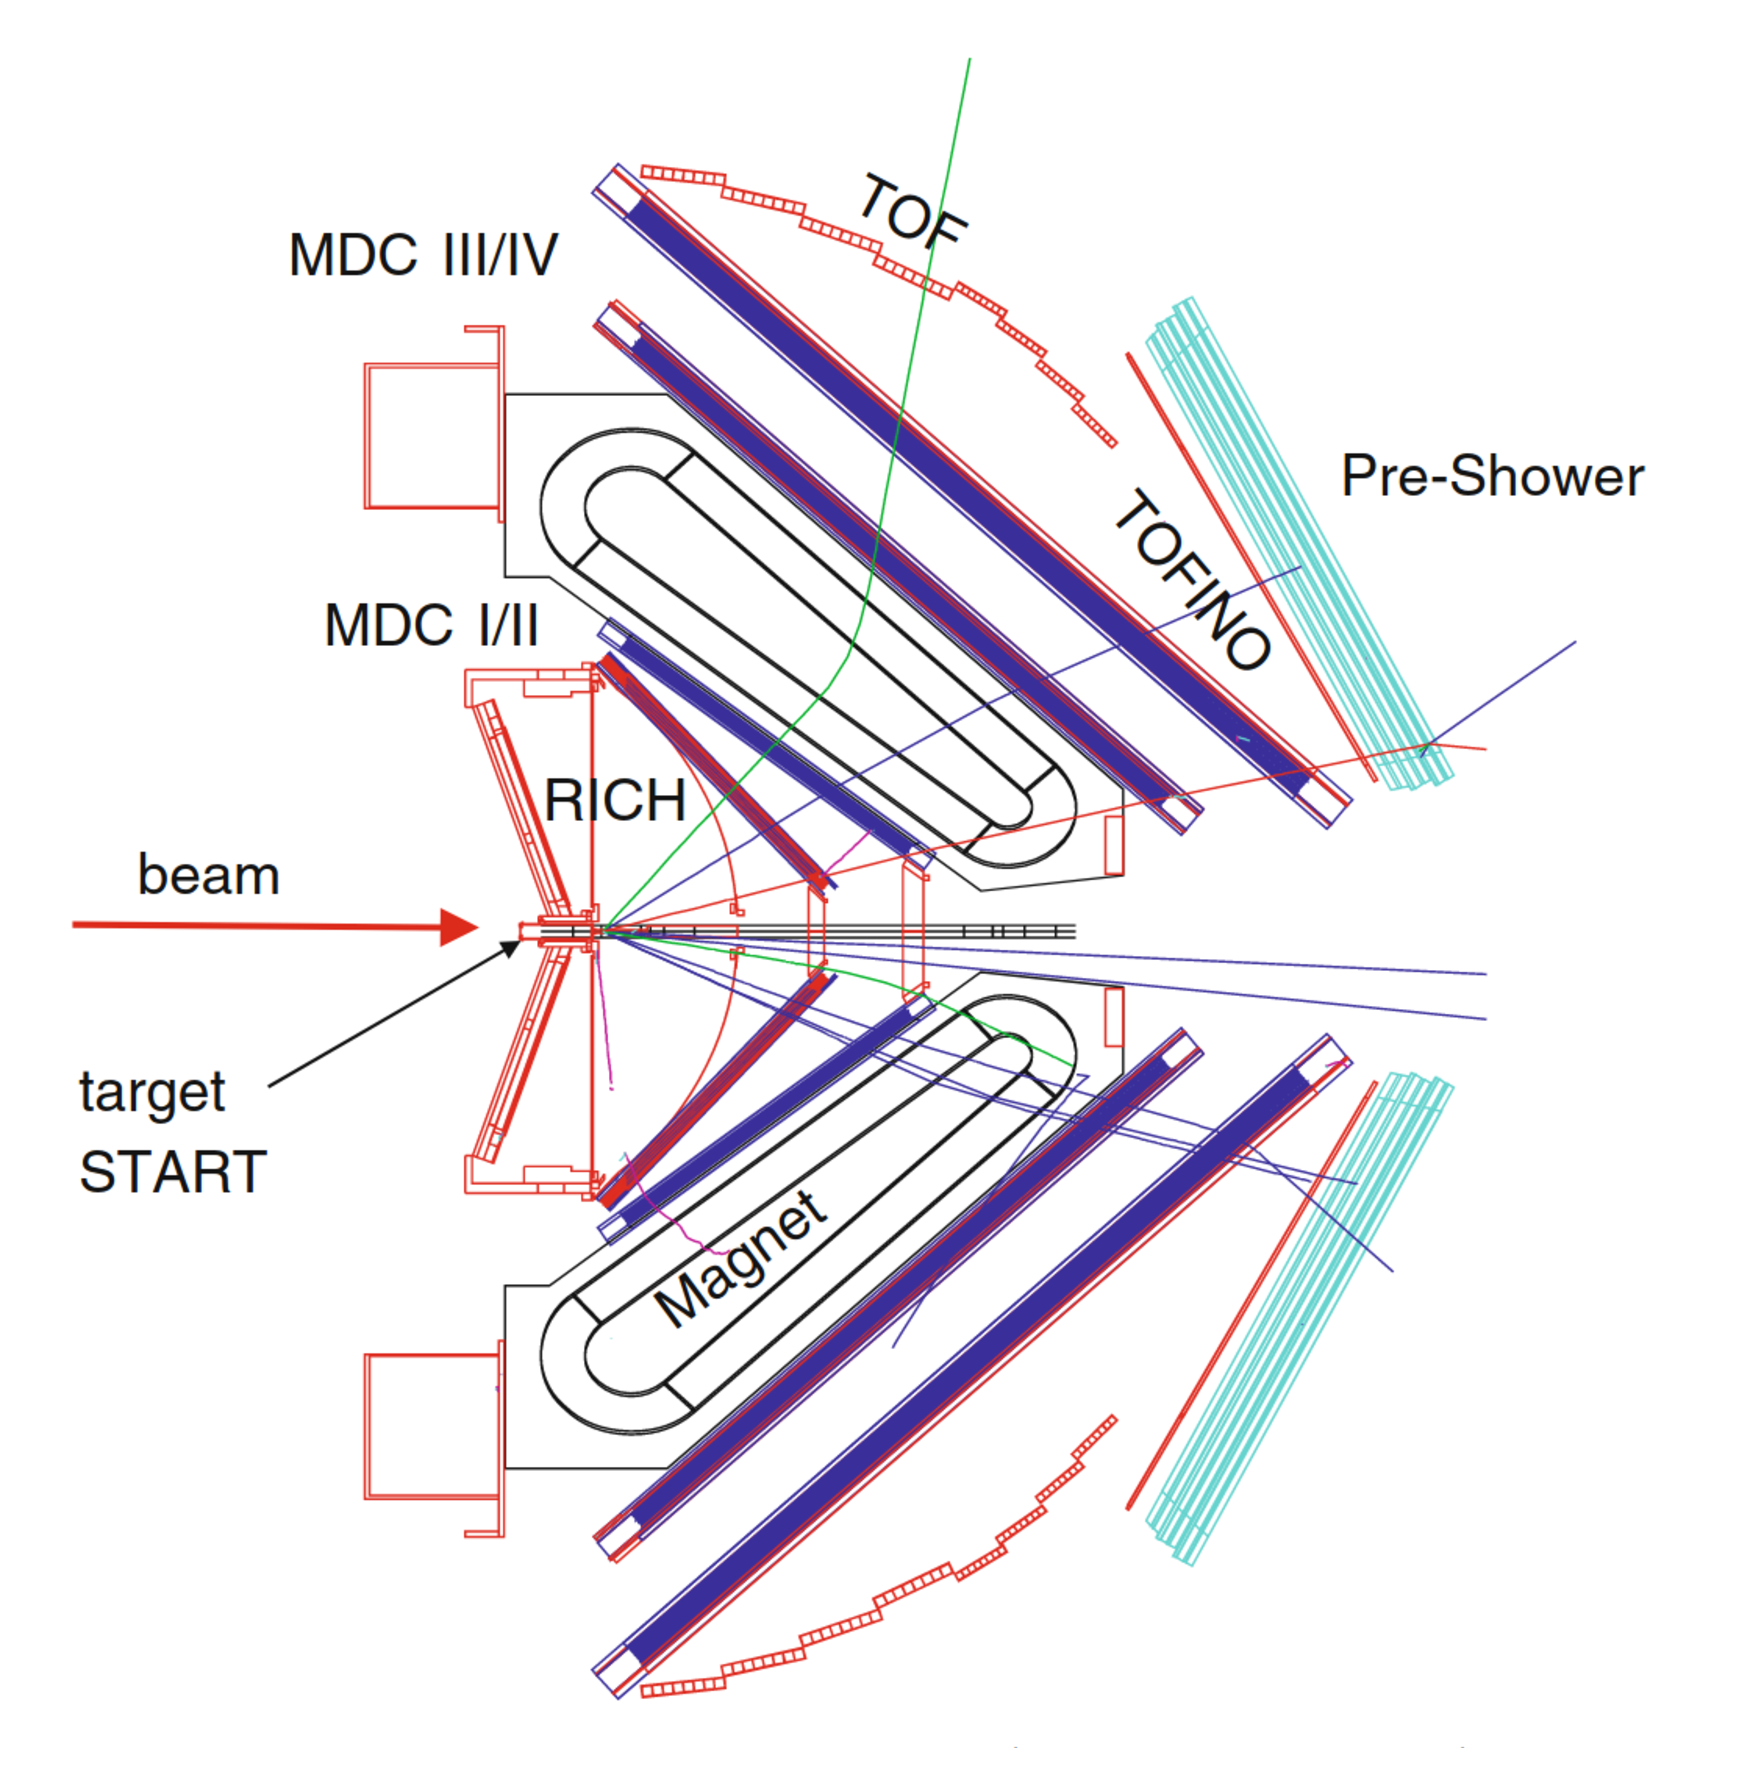
\includegraphics[width=0.7 \linewidth]{Chapter_detector/detektor.eps}
  \caption{The HADES - \cs through the detector. All essential sub-systems used during pp and pNb experiment are visible in the picture. The picture from \cite{Agakishiev:2009am}.}
\end{figure}

\section{Tracking system}
The HADES tracking system bases on four sets of a drift chambers. Two before and two after a magnetic field. First set is called inner MDC, the second outer MDC. Each single drift chamber has a trapezoidal shape and consist of 13 layers of wires. They create 6 layers of a drift cells. A shape of the sells and the wires density was optimized to get the best momentum resolutions.

In between inner- and outer-MDC the \textbf{I}ron\textbf{L}ess \textbf{S}uperconducting Electron (ILSE) Magnet is located. It consist of six superconducting coils, which produce a toroidal magnetic field of 3.6 T inside the coils. The operational current can vary from 0 to 3500 A. 

The magnetic field produced by ILSE bends particles' tracks what allows for a momentum reconstruction. Tracks reconstructed in inner- and outer-MDCs have to be matched together. A dedicated algorithm for this purpose was developed by HADES collaboration and uses solutions of an equation of motion obtained by Runge-Kutta metode.

\section{PreShower and META detectors}
During a pp@3.5~GeV and pNb@3.5~GeV experiments the HADEs culminated with a META (\textbf{M}ultiplicity \textbf{E}lectron \textbf{T}rigger \textbf{A}rray) detector. The META system played two main roles: provided en information about particles time of flight and was utilized as a source for a multiplicity trigger. The detector consisted of two sub-systems: a TOF for polar angles from 44 to 88 degrees and a TOFino angles from 18-45 degree. They also differed by a time resolution $\sigma_{TOF}\approx~150~\mathrm{ps}$, $\sigma_{TOFino}\approx~450~\mathrm{ps}$. The main difference between these detectors was in space resolution properties. Each strap of the TOF detector has a readout at both ends of scintilator. It allows for an estimation of an interaction place base on a time difference between signal arrival in both ends of the detector. Due to economical circumstances the TOFino detector has much smaller granulation and a reed out was installed an one end of each strap. It caused much worse space resolution for the TOFino than for the TOF detector.

An information about interaction point for TOFino detector is given by PreShower detector, located behind the TOFino. Its main purpose was to enhance a capability for lepton identification for polar angles below 45$\deg$. In principle it was a thin, three layer, electromagnetic calorimeter, although it didn't take a role of a calorimeter. It was too thin to fully stop leptons, but thick enough to observe a beginning of an electromagnetic cascade. The detector consisted of three drift chambers layered with two led plates and an energy deposited in each drift chamber was registered. In case of leptons total charge collected for 2nd and 3rd are higher than for 1st. For hadrons deposited energy does not change with detector layer. The detector was used for both: leptons identification and lepton trigger (LVL2).

\section{RICH detector}
The \textbf{R}ing \textbf{I}maging \textbf{CH}erenkov detector is the main tool for $\epem$ identification for the HADES. The detector active area surrounds target area and it is filled by a radiator gas ($\mathrm{C}_4 \mathrm{F}_{10}$). A refractive index gives a threshold speed for a Cherenkov radiation production $\gamma_{thr} =18$. For projectile energies delivered by the SIS18 only particles able to exceed the threshold are electrons end positrons. Passing across the radiator they produce a cone of a Cherenkov light. Then, the light is reflected by a spherical mirror and detected by a pad plane located upstream a beam. An special algorithm called ''ring finder'' \cite{hades_RICH} reconstructs Cherenkov light rings from a pattern of fired pads. A reconstructed ring position is matched with track from MDC to assign information about a leptonic character to proper track.  The detector is completely ''hadron blind'' what means that no hadron can give an signal in it. In 2019 the RICH was updated by a new readout system, described more detailed in next section. 
\begin{figure}
  \centering
  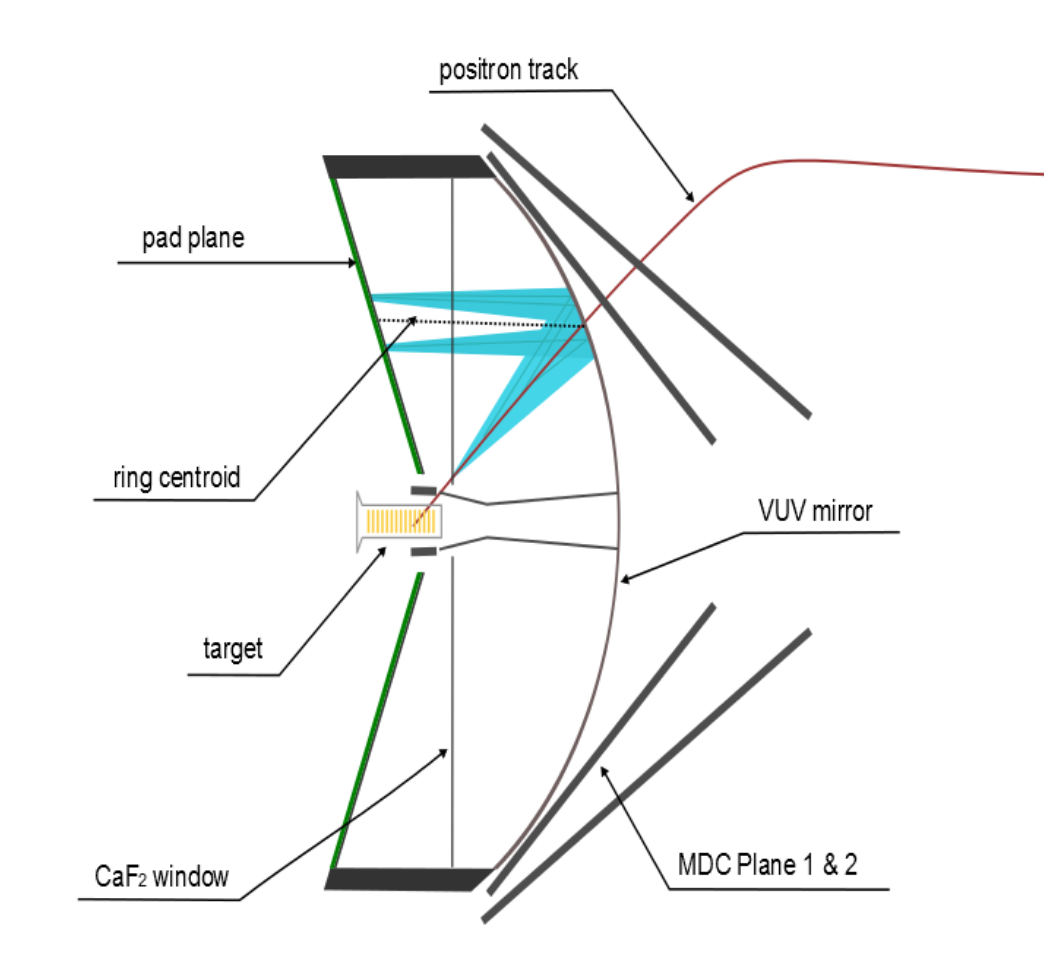
\includegraphics[width=0.6 \linewidth]{Chapter_detector/RICH.png}
  \caption{The \cs of the RICH detector.}
\end{figure}
\section{The HADES upgrades}
\label{chapter:HADES_upgrades}
Currently HADES is intensively upgraded to face a new physical program. A brand new \textbf{E}lectromagnetic \textbf{CAL}orimeter \cite{FAIRness:Hudoba,FAIRness:Shabanov} and a new RICH readout system have been already installed and tested during campaign with Ag+Ag collisions. In addition a new \textbf{F}or\textbf{W}ard \textbf{DET}ector \cite{FAIRness:Malige} was installed in 2020. It will extend the HADES acceptance to very forward angles, between~$0.6^{\circ}$~and~$7^{\circ}$. One of the main reasons for FwDet development are hyperon studies. This detector will significantly enhance the acceptance for $\Lz$ reconstruction, since momentum conservation causes the proton from $\Lambda$ decay tend to be emitted at small polar angles.Detail about new possibilities for hyperon research opened by the FwDet are presented in. \ref{chapter:simulations}.
\begin{figure}[ht]
  \centering
  \includegraphics[width=0.6 \linewidth]{Chapter_detector/HADES.png}
  \caption{The HADES detector with new updates. Parts labeled by a red font have been installed in 2019 or later and are discussed in following subsection.}
\end{figure}
\subsection{The Forward Detector}
\label{subsec:FwDet}
In many studies, especially devoted to hyperons' decays the forward angles play very important role. The HADES detector for a quite long time did not have a possibility to register particles emitted into polar angle below 10 degree. That situation is changing because of a new \textbf{F}or\textbf{w}ard~\textbf{Det}ector build in a collaboration between Jagiellonian University Cracow, Institut de Physique Nucléaire d'Orsay and Forschungszentrum Jülich.

\begin{figure}[hb]
  \centering
  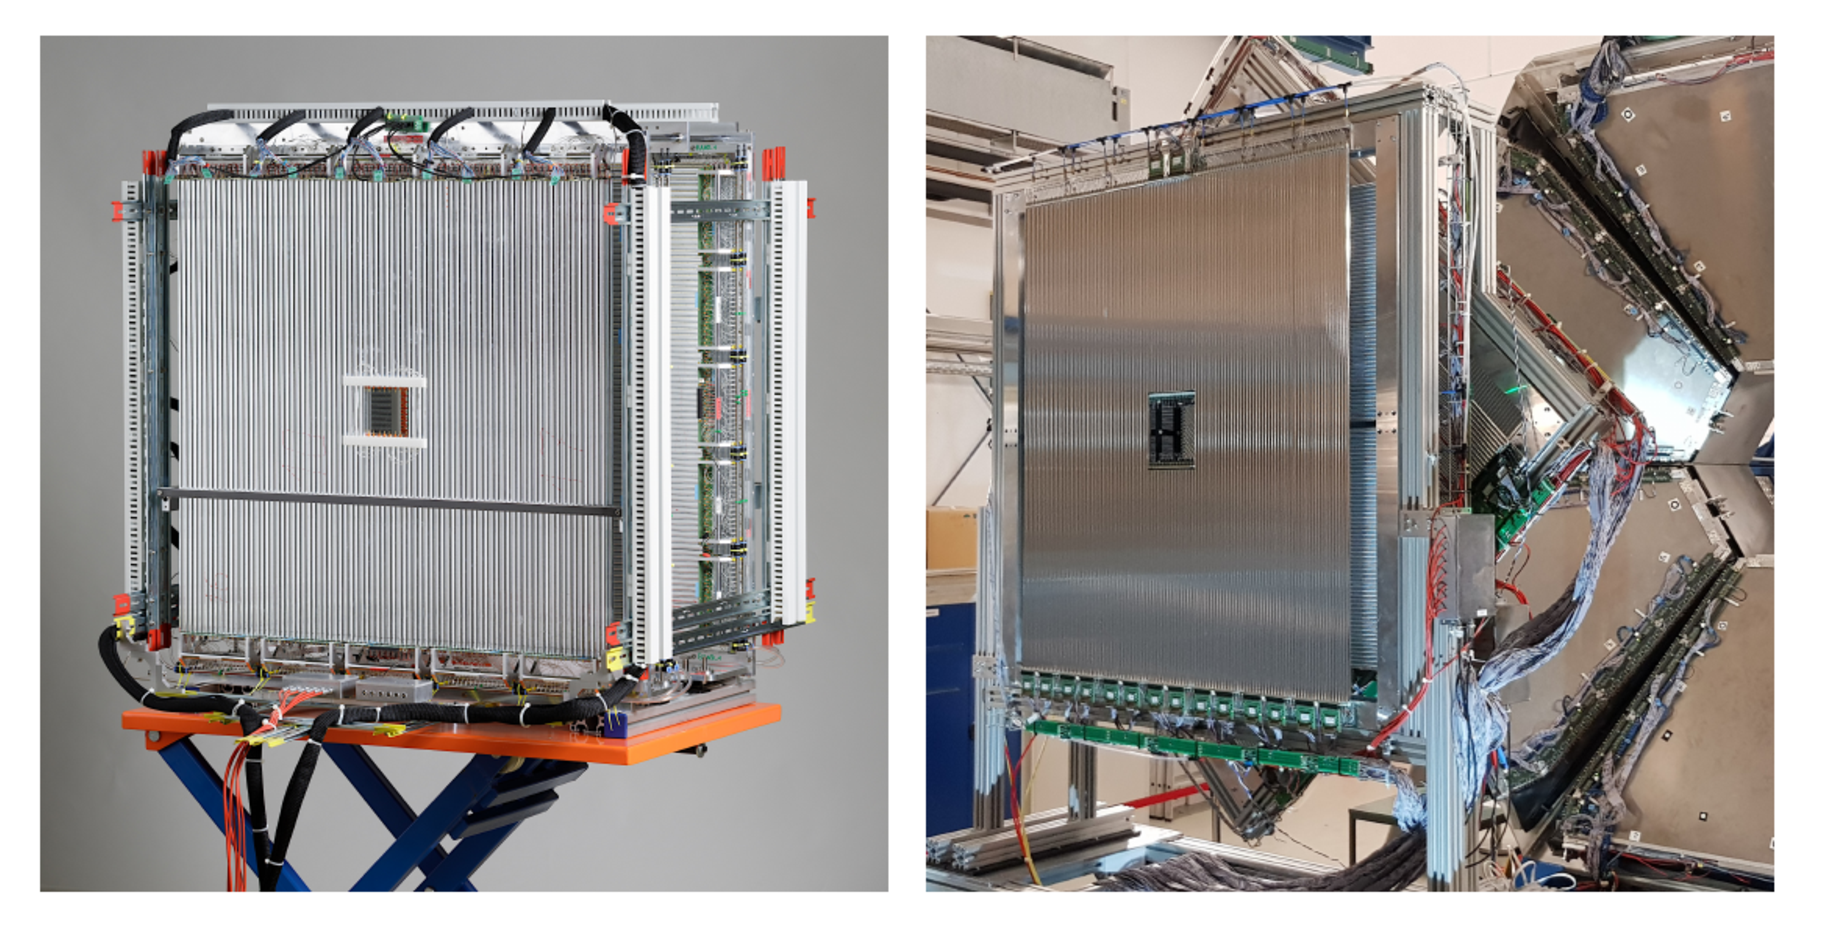
\includegraphics[width=0.6 \linewidth]{Chapter_detector/FwDet.eps}
  \caption{Both tracking stations of the FwDet detector, left: STS1, right: STS2}
\end{figure}

FwDet is a tracking detector consist of two tracking stations: STS1 and STS2. They are made utilizing the same technology as planned forward detector for the PANDA experiment. Each of the stations consist of a set of straws filled by a ArCO$_2$ gas under a pressure of 2 bar. Straws are collected end glued together in modules, 32 straws each. Such a structure, together with overpresure, makes the detector self-supporting. The operational voltage between an anode wire, which is located in center of each straw, and cathode a straw is 1800 V. It resulting a gas gain $5 \cdot 10^4$ and maximum drift time 130 ns. The spatial resolution for single straw is 0.13 mm [ref].

In the STS1 straws are organized in four double-layers aligned by an inclination $0\deg, 90\deg, 0\deg, 90\deg$. The STS2 also consist of four layers but, for better tracking abilities two of them are twisted by $45\deg$. A similar solution was not possible for the STS1 because of lack of a space in ECAL create. The STS2 ends by an RPC detector which provides a precise information about time-of-flight for each track.

Besides a hardware development, track reconstruction and tracking algorithms were developed in Jagiellonian University. A track reconstruction bases on an assumption that between the stations there is no magnetic field. It meas that all tracks are straight lines, and only kinematic variable is a time of flight measured by RPC. It means that it is impossible to make an unambiguous identification of detected particles and some kind of information have to be assumed. The reconstruction procedure using FwDet is described more detailed in \ref{chapter:simulation_identyfication}. Details of the detector structure and prepared software are described in [artykul Rafala]. 
\subsection{RICH update}

\subsection{Electromagnetic calorimeter}
In 2018 first four sector of a new \textbf{E}lectromagnetic \textbf{CAL}orimeter was commisioned. As a target ECAL is going to consist of six toroidal sectors, that reflects a generlal HADES symmetry. They will be assembeled at the end of the detector and will replace pre-shower detector. In final configuration, with all six sectors the calorimeter will have almost full azimuntal covering and 12 to 45 degree fovering in animuntal angle. Its main purpose is to extend the HADES capabilites by a photon detection - a capability complemantary to di-lepton reconstruction provided by RICH. It will allow for a reconstruction of a netral mesons and barionic resosnanses' photo-decays.

\begin{figure}[ht]
  \centering
  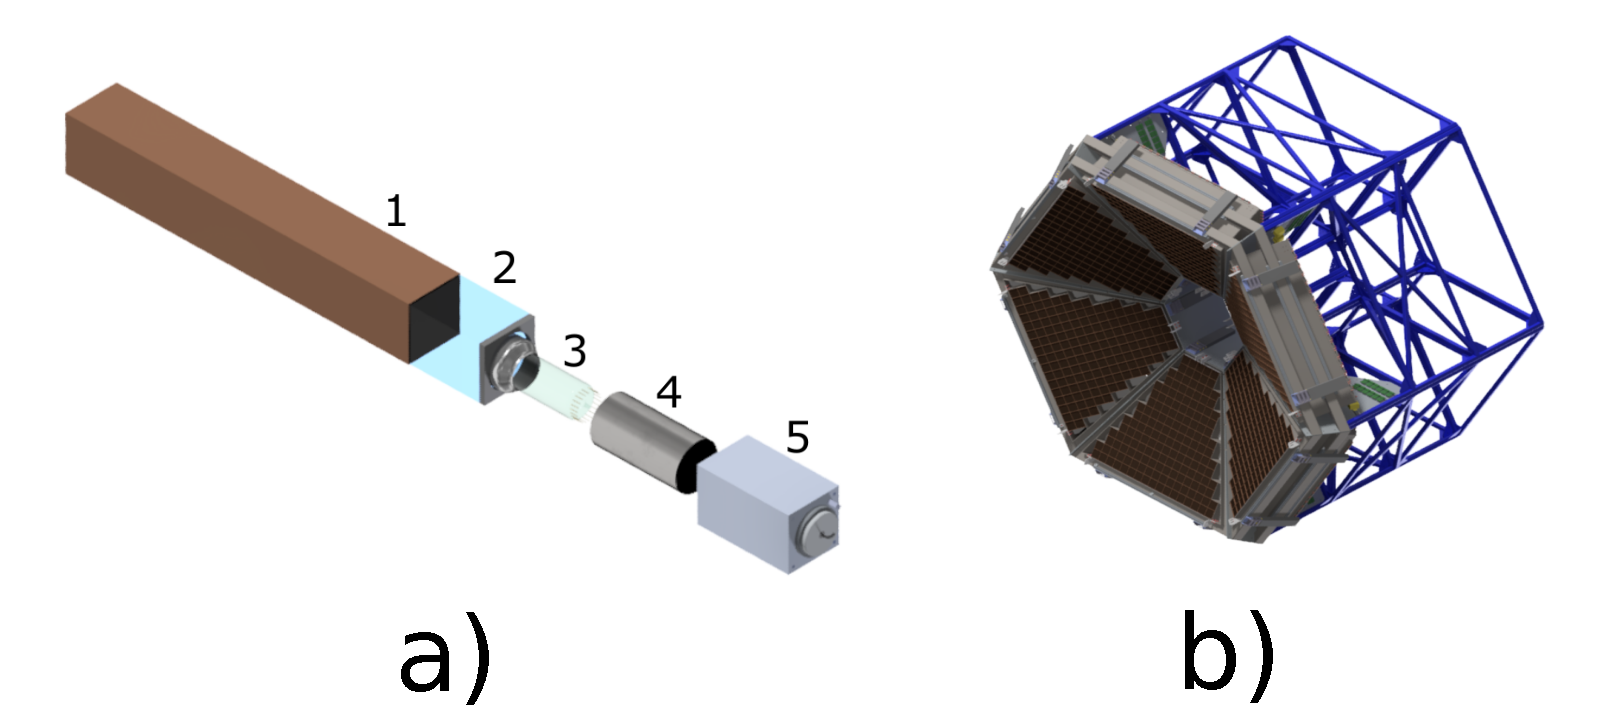
\includegraphics[width=0.9 \linewidth]{Chapter_detector/ECAL.eps}
  \caption{The ECAL detector: a) single module, b) entire aparatus. Each module sonsist of following parts: 1-brass envelope, 2-lead-glass radiator, 3-photomultiplayer, 4-magnetic shielding, 5-aluminiumhousing for PMT. The figure from \cite{FAIRness:Hudoba}.}
\end{figure}


The calorimeter constis of 163 modules, each of them composed of a brass envelope a lead-glass prism and a photomultiplayer enclosed in MUMETALL shielding. A high energy photon propagating throu a glass causes an electromagnetic cascade. Charged particles from the cascade, mostly $\epem$ pairs, traveling across the led-glass produce a cherenkov light. Next, cherenkov-light photons are detected by a photomultiplayer at the end of the module. Designed resolution, verivied by experiment, is $\frac{\Delta E}{E}=5.5\%$ for 1 GeV photons.


